\documentclass[14pt]{beamer}

\usetheme{CambridgeUS}
\setbeamercolor{title}{bg=red!65!black,fg=white}
\setbeamertemplate{title page}[default][colsep=-4bp,rounded=true]
\setbeamercolor{author}{bg=white,fg=red!65!black}
\setbeamercolor{date}{bg=white,fg=red!65!black}
\setbeamertemplate{itemize items}[default]
\setbeamertemplate{enumerate items}[default]
\setbeamertemplate{section in toc}[circle]
\setbeamertemplate{subsection toc}[circle]
\setbeamertemplate{blocks}[rounded][shadow=false]

\usepackage{braket}

%\newcommand{\braket}[1]{\ensuremath{\left | #1 \right \rangle}}

\usepackage{hyperref}
\usepackage{verbatim}
\usepackage{tikz}
\usepackage[utf8]{inputenc}
\usepackage{amsmath}
\usepackage{amsfonts}
\usepackage{amssymb}
\usepackage{graphicx}
\author{William Bernoudy}
\title[Theory and Applications of QC]{\textbf{Theory and Applications of Quantum Computing}}
\setbeamercovered{transparent} 
%\setbeamertemplate{navigation symbols}{} 
%\logo{} 
%\institute{} 
%\date{} 
%\subject{} 

\makeatletter
\setbeamertemplate{footline}
{
  \leavevmode%
  \hbox{\fontsize{7}{13}\selectfont%
  \begin{beamercolorbox}[wd=.333333\paperwidth,ht=2.25ex,dp=1ex,center]{author in head/foot}%
    \usebeamerfont{author in head/foot}\insertshortauthor
  \end{beamercolorbox}%
  \begin{beamercolorbox}[wd=.333333\paperwidth,ht=2.25ex,dp=1ex,center]{title in head/foot}%
    \usebeamerfont{title in head/foot}\insertshorttitle
  \end{beamercolorbox}%
  \begin{beamercolorbox}[wd=.333333\paperwidth,ht=2.25ex,dp=1ex,right]{date in head/foot}%
    \usebeamerfont{date in head/foot}\insertshortdate{}\hspace*{1em}% original: 2ex
    \insertframenumber{} / \inserttotalframenumber\hspace*{1ex}% original: 2ex
  \end{beamercolorbox}}%
  \vskip0pt%
}
\makeatother

\setbeamerfont{footline}{size=\fontsize{10}{11}\selectfont}
\setbeamercovered{invisible}

\let\olditem\item
\renewcommand{\item}{%
\olditem\vspace{10pt}}

\begin{document}
\usebackgroundtemplate{%
  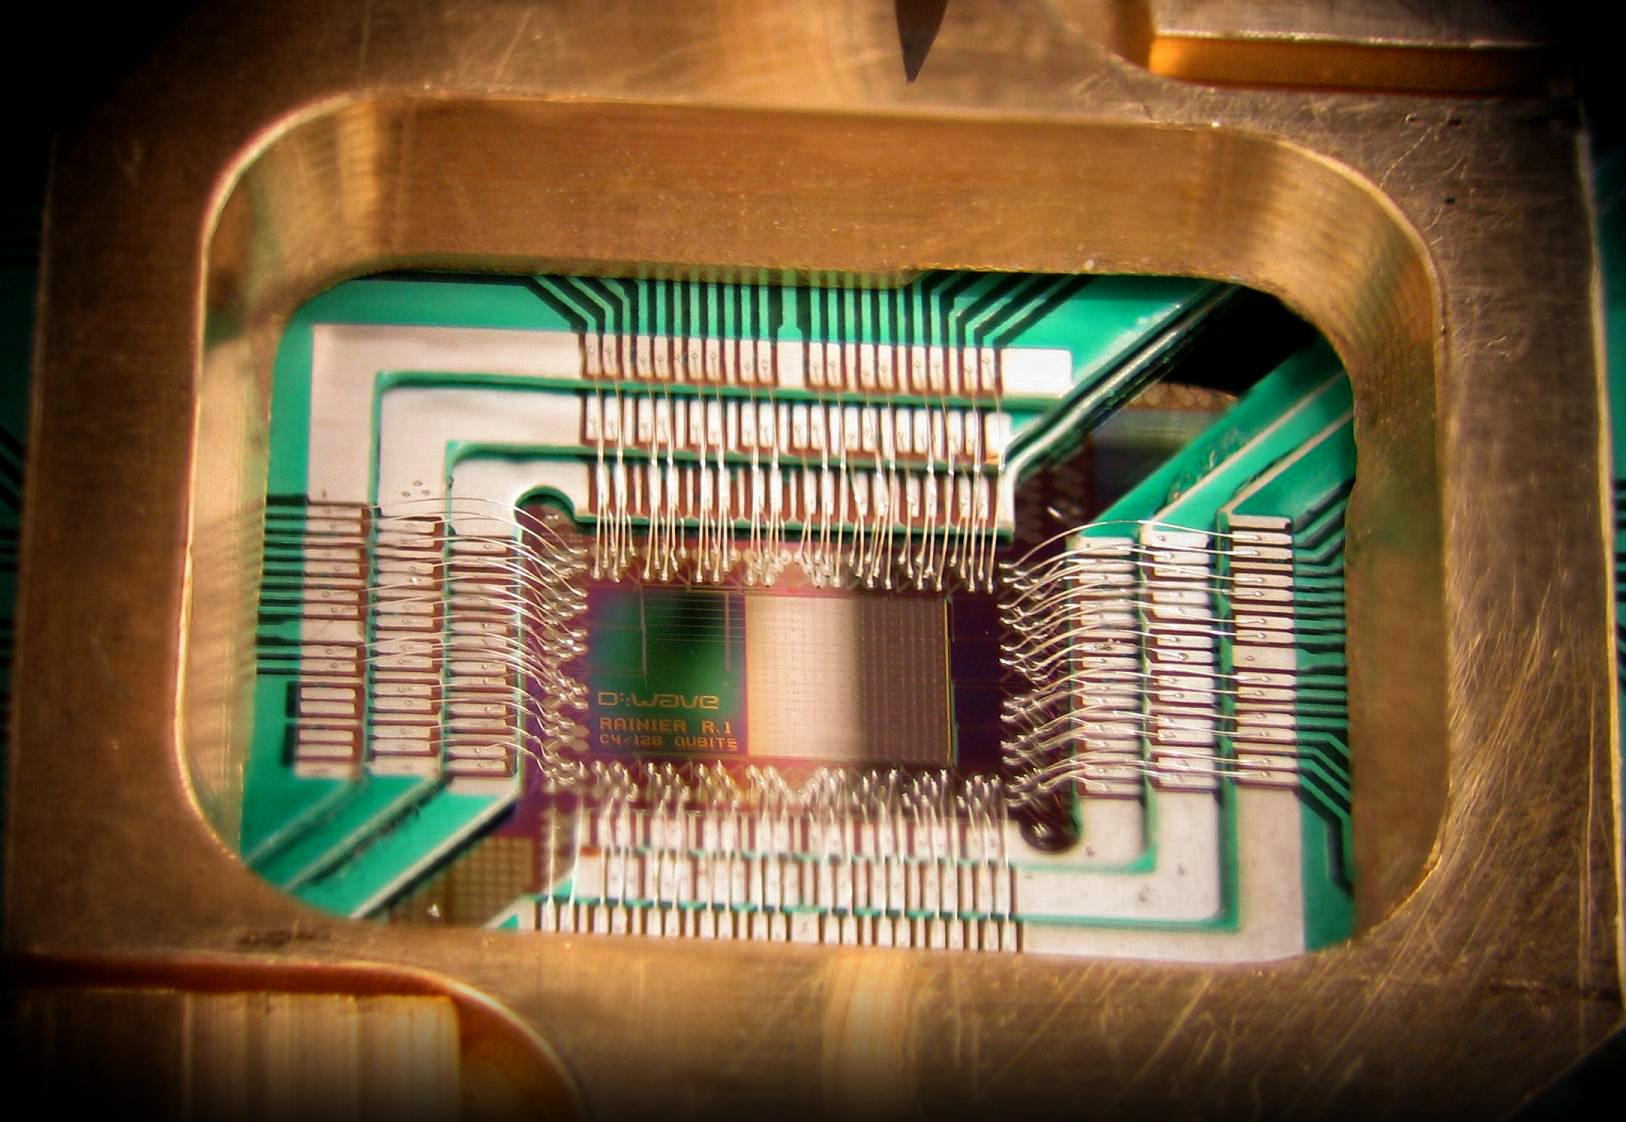
\includegraphics[width=\paperwidth,height=\paperheight]{../resources/images/dwave_chip.jpg}} 
  
\begin{frame}
\titlepage
\end{frame}

\usebackgroundtemplate{}

%\begin{frame}
%\tableofcontents
%\end{frame}

\begin{comment}
\begin{frame}{About me}
\begin{itemize}
	\item 4th year at Quest
	\item My Question is ``What are the applications of quantum computing?"
	\item I interned at D-Wave Systems and got to run problems on a real quantum computer
\end{itemize}
\end{frame}
\end{comment}

\begin{comment}
\begin{frame}{Goals for this workshop}
\begin{itemize}
	\item Appreciate the math that models quantum computing
	\item Get an intuitive understanding of how they work, play with a fun tool
	\item Think about applications
\end{itemize}
\end{frame}
\end{comment}

\section{What is quantum computing?}
\begin{frame}{What do we mean by \textit{quantum}?}
\begin{itemize}
	\item Quantum mechanics
	\item Quantum phenomena: superposition, 	entanglement, tunneling 
\end{itemize}
\begin{center}
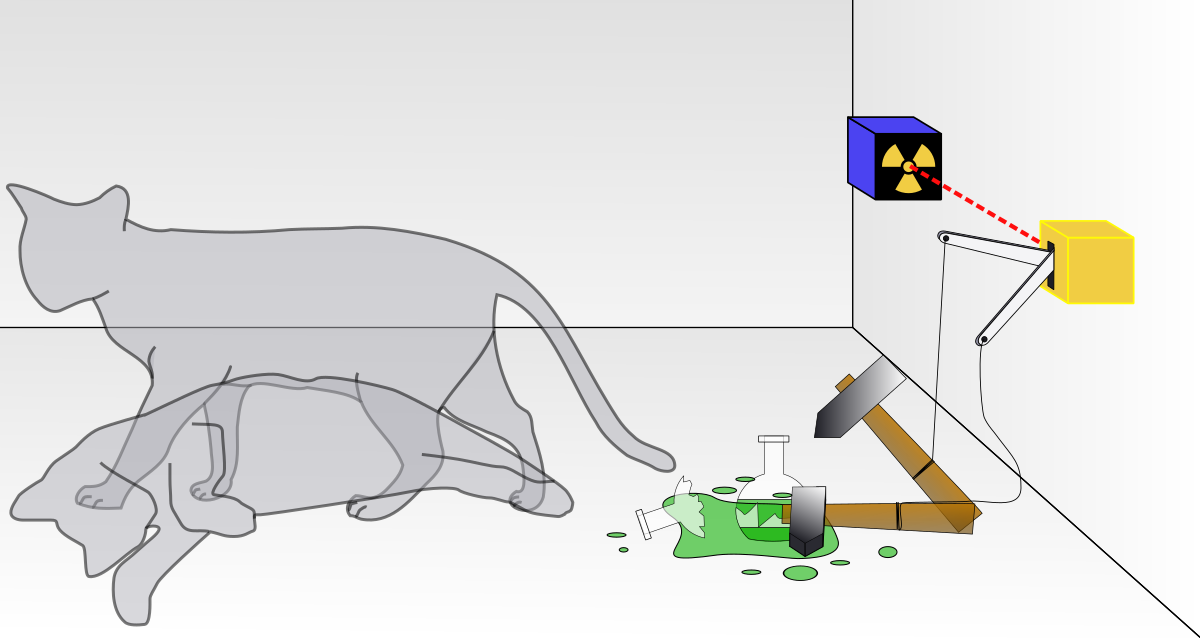
\includegraphics[scale=0.15]{../resources/images/Schrodingers_cat.png}\\
{\tiny By Dhatfield - Own work, CC BY-SA 3.0, https://commons.wikimedia.org/w/index.php?curid=4279886\par}
\end{center}
\end{frame}

\begin{frame}{What is quantum computing?}
\begin{itemize}
	\item Take advantage of quantum phenomena	
	\item Specialized, better than classical computers at certain types of problems
	\item Extremely hard to build physical realizations
\end{itemize}
\end{frame}

\begin{comment}
\begin{frame}{ Quantum computing models}
\begin{itemize}
\item Universal quantum computers
\item Quantum annealing
\item Many possible physical realizations
\end{itemize}
\end{frame}
\end{comment}

\subsection{Classical computing}
\begin{comment}
\begin{frame}{Bits as vectors}
\begin{itemize}
	\item Bit has two states: 0 and 1
	\item We can model each state with a vector
\end{itemize}
$$\ket{0} = \begin{pmatrix}1\\ 0\end{pmatrix} \quad \ket{1}=\begin{pmatrix}0\\ 1\end{pmatrix}$$
\end{frame}
\end{comment}

\begin{frame}{Modeling bits}
\begin{columns}[T]
	\begin{column}{.6\textwidth}
		\begin{block}{}
			\begin{itemize}
				\item Bit has two states: 0 and 1
				\item $b = \ket{0}$ or $\ket{1}$
				\item Classical computation amounts to flipping between these states
			\end{itemize}
    	\end{block}
	\end{column}
	\begin{column}{.05\textwidth}
	\end{column}	
	\begin{column}{.3\textwidth}
    	\begin{block}{}
			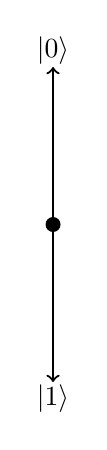
\begin{tikzpicture}[]
				\draw[<-, thick] (0,2) -- (0,0) node[near start, above, shift={(0, 0.4)}] {$\ket{0}$}; %{$\ket{0}} = \begin{pmatrix}1\\ 0\end{pmatrix}$};
				\filldraw (0,0) circle (2.5pt);
				\draw[->, thick] (0,0) -- (0,-2) node[near end, below, shift={(0, -0.4)}] {$\ket{1}$}; %{$\ket{1}} %=\begin{pmatrix}0\\ 1\end{pmatrix}$};
			\end{tikzpicture}
		\end{block}
	\end{column}
\end{columns}
\end{frame}

\begin{comment}
\begin{frame}{System vectors for bits}
\begin{itemize}
	\item Computation happens on more than one bit at once
	\item We can also represent multi-bit systems with a single vector
	\item $\ket{00} = \begin{pmatrix} 1 \\ 0 \\ 0 \\ 0 \end{pmatrix} \quad \ket{10} = \begin{pmatrix} 0 \\ 0 \\ 1 \\ 0 \end{pmatrix} \quad \ket{111} = \begin{pmatrix} 0 \\ 0 \\ 0 \\ 0 \\ 0 \\ 0 \\ 0 \\ 1\end{pmatrix}$
\end{itemize}
\end{frame}
\end{comment}

\subsection{Universal quantum computer}
\begin{frame}{Qubits}
\begin{columns}[T]
	\begin{column}{.5\textwidth}
		\begin{block}{}
			\begin{itemize}
				\item Analogous to the bit
				\item Infinite possible states
				\item $\ket{q} = a_0 \ket{0} + a_1 \ket{1}$
				%\item<3-> Constraint: $|a_0|^2 + |a_1|^2 = 1$
				%\item $\ket{\psi} = ae^{i\theta}\ket{0} + be^{i\phi}\ket{1}$
				%\item $1 = a^2(\cos^2{\theta} + \sin^2{\theta}) + b^2(\cos^2{\phi} + \sin^2{\phi})$
				%\item $a^2 + b^2 = 1$
			\end{itemize}
    	\end{block}
	\end{column}
	\begin{column}{.5\textwidth}
    	\begin{block}{}
		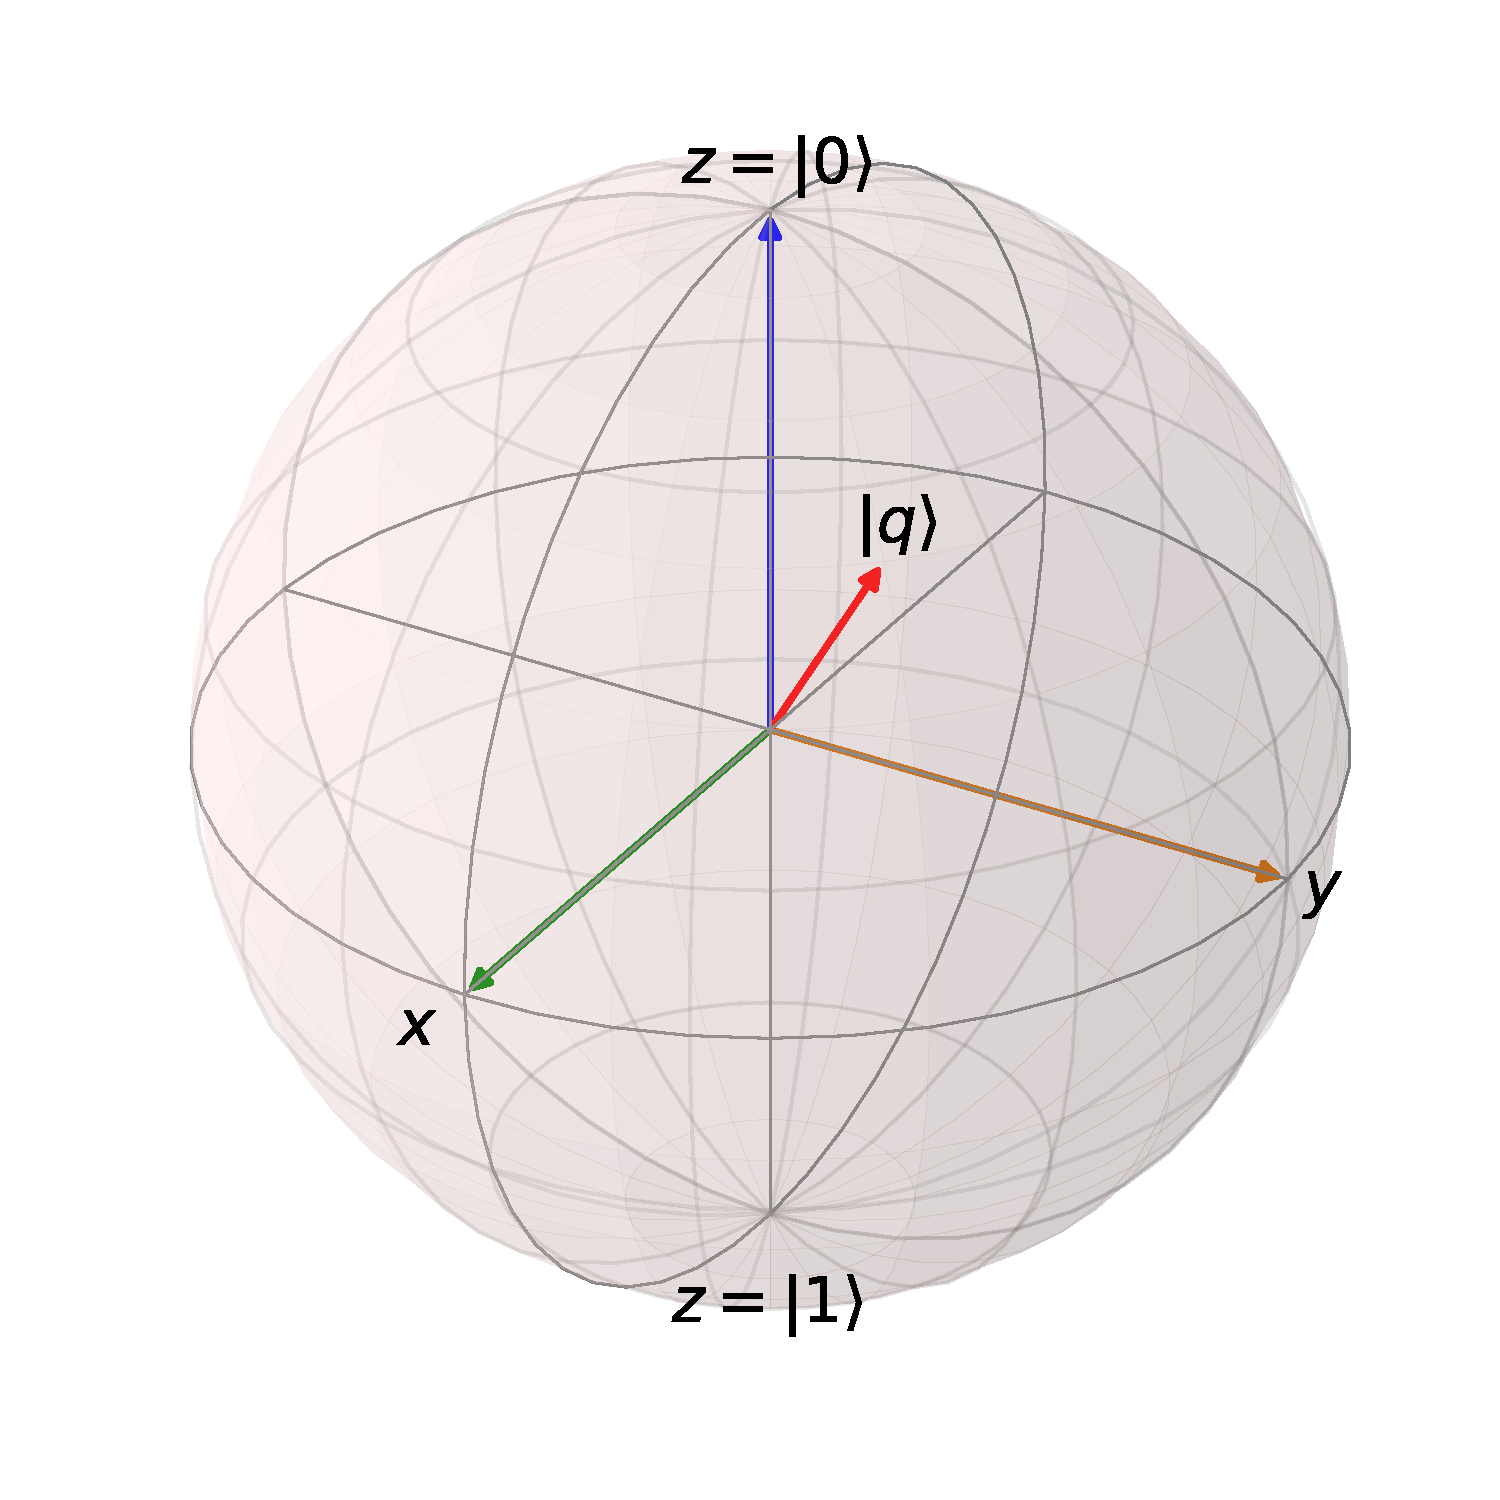
\includegraphics[width=1\textwidth]{../resources/pdfs/custom_Bloch_sphere.pdf}
	\end{block}
	\end{column}
\end{columns}
\end{frame}

\begin{frame}{Qubits}
\begin{itemize}
	\item With bits, we can always ``examine" them to see their state
	\item For qubits, measurement collapses their state
	\item Qubits are probabilistic 
\end{itemize}
\end{frame}

\subsection{Universal quantum computer}
\begin{frame}{Qubits}
\begin{columns}[T]
	\begin{column}{.5\textwidth}
		\begin{block}{}
			\begin{itemize}
				\item $\ket{q} = a_0 \ket{0} + a_1 \ket{1}$
				%\item<3-> Constraint: $|a_0|^2 + |a_1|^2 = 1$
				\item Probability of \\ observing \\ 
						$\ket{0}$: $|a_0|^2$ \\
						$\ket{1}$: $|a_1|^2$
				%\item $\ket{\psi} = ae^{i\theta}\ket{0} + be^{i\phi}\ket{1}$
				%\item $1 = a^2(\cos^2{\theta} + \sin^2{\theta}) + b^2(\cos^2{\phi} + \sin^2{\phi})$
				%\item $a^2 + b^2 = 1$
			\end{itemize}
    	\end{block}
	\end{column}
	\begin{column}{.5\textwidth}
    	\begin{block}{}
		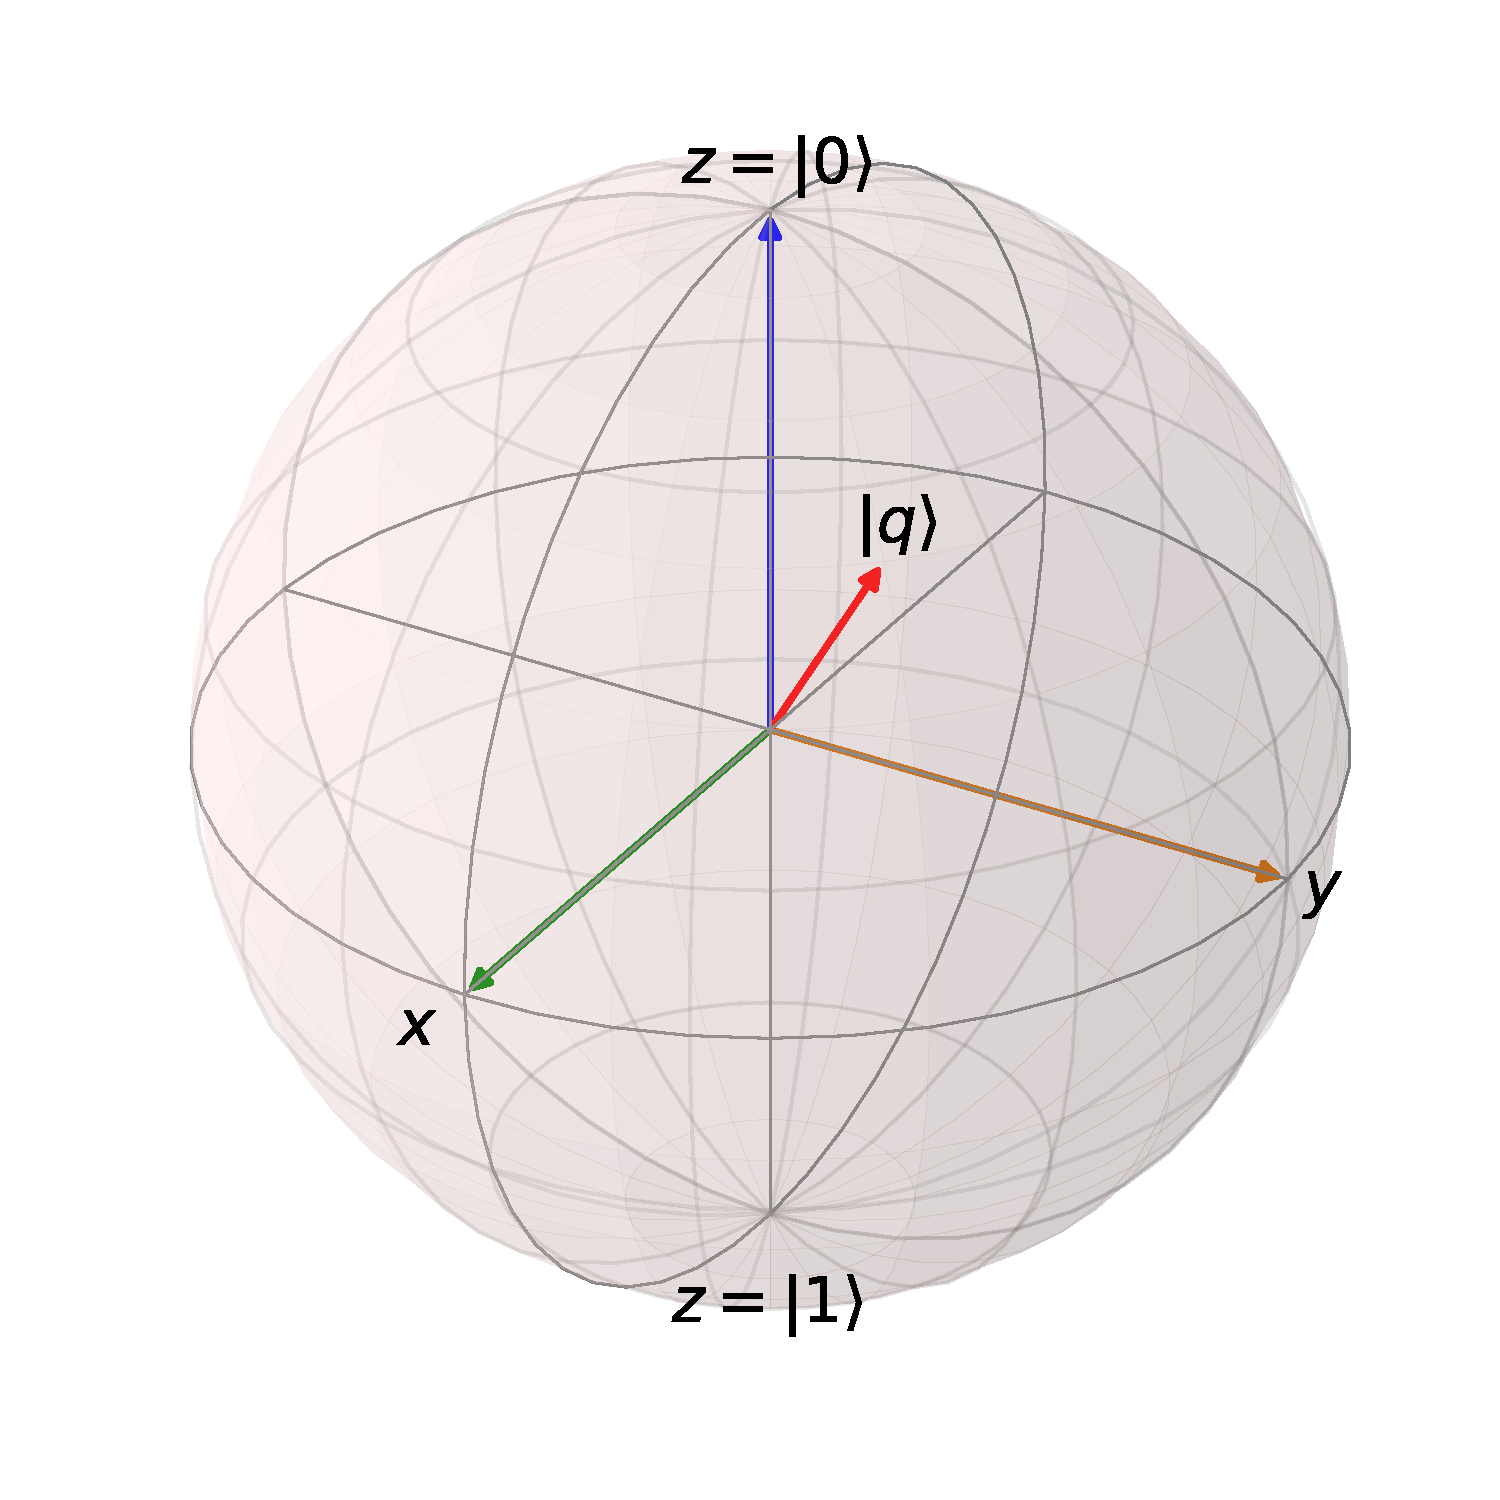
\includegraphics[width=1\textwidth]{../resources/pdfs/custom_Bloch_sphere.pdf}
	\end{block}
	\end{column}
\end{columns}
\end{frame}

\begin{comment}
\begin{frame}{Quantum system state vector}
\begin{itemize}
	\item Just as with classical computers, we can have multiple qubits with longer state vectors
	\item \small{$\ket{\Psi} = \begin{pmatrix} \alpha_0 \\ \alpha_1 \\ \alpha_2 \\ \alpha_3 \end{pmatrix} \quad \ket{\Psi} = \begin{pmatrix} \alpha_0 \\ \alpha_1 \\ \alpha_2 \\ \alpha_3 \\ \alpha_4 \\ \alpha_5 \\ \alpha_6 \\ \alpha_7 \end{pmatrix}$}
	\item Restraint: $|\alpha_0|^2 + |\alpha_1|^2 + |\alpha_2|^2 + ... = 1$
\end{itemize}
\end{frame}
\end{comment}

\begin{frame}{Quantum gates}
\begin{itemize}
	\item To carry out actual computation, we apply \textit{gates} to the qubits
  	\item A gate is a function which changes the qubits' states in a predictable manner
  	\item Common gates ``rotate" the qubit's state on the Bloch sphere
	%\item Each gate can be represented as a matrix
	%\item The following system state is a result of the multiplying the gate by the previous state vector
\end{itemize}
\end{frame}

\begin{frame}{Examples of gates}
\begin{itemize}
	\item Pauli-x or NOT gate ($\sigma_x$): $\begin{pmatrix} 0 & 1 \\ 1 & 0 \end{pmatrix}$
	\item Pauli-z gate ($\sigma_z$): $\begin{pmatrix} 1 & 0 \\ 0 & -1 \end{pmatrix}$
	\item Hadamard ($H$): $\frac{1}{\sqrt{2}}\begin{pmatrix} 1 & 1 \\ 1 & -1 \end{pmatrix}$
\end{itemize}
\end{frame}

\begin{frame}{Applying gates}
\begin{itemize}
	\item Start with a state vector $\ket{\Psi} = \begin{pmatrix}0 \\ 1\end{pmatrix}$
	\item Applying a Pauli-x gate: $\sigma_x \ket{\Psi} = \begin{pmatrix} 0 & 1 \\ 1 & 0 \end{pmatrix}\begin{pmatrix}0 \\ 1\end{pmatrix} = \begin{pmatrix}1 \\ 0\end{pmatrix}$
	\item Applying a Hadamard: $H \ket{\Psi} = \frac{1}{\sqrt{2}}\begin{pmatrix} 1 & 1 \\ 1 & -1 \end{pmatrix}\begin{pmatrix}0 \\ 1\end{pmatrix} = \frac{1}{\sqrt{2}}\begin{pmatrix}1 \\ -1\end{pmatrix} = \begin{pmatrix}\frac{1}{\sqrt{2}} \\ -\frac{1}{\sqrt{2}}\end{pmatrix}$
	
\end{itemize}
\end{frame}

\begin{comment}
\begin{frame}{Recap}
\begin{itemize}
	\item Bits only have two states, qubits can point anywhere on the Bloch sphere
	\item We can rotate and manipulate the qubit's state with quantum gates, but can't ever measure the state directly
\end{itemize}
\end{frame}
\end{comment}

\begin{comment}
\section{Building an intuition}
\begin{frame}{Building an intuition}
Let's try out a fun tool! http://algorithmicassertions.com/quirk (Thank you Craig Gidney!)
\begin{itemize}
	\item Pauli rotation gates: \href{http://algorithmicassertions.com/quirk\#circuit={"cols":[["Bloch"],["X"],["Bloch"]]}}{link}
	\item Hadamard gate: \href{http://algorithmicassertions.com/quirk\#circuit={"cols":[["Bloch"],["H"],["Bloch"]]}}{link}
	\item Controlled-NOT gate: \href{http://algorithmicassertions.com/quirk\#circuit={"cols":[["Bloch","Bloch"],["\%E2\%80\%A2","X"],["Bloch","Bloch"],["X"],["Bloch","Bloch"],["\%E2\%80\%A2","X"],["Bloch","Bloch"]]}}{link}
\end{itemize}
\end{frame}
\end{comment}

\begin{comment}
\section{Applications}
\begin{frame}{What are the applications?}
\begin{itemize}
	\item QC doesn't violate the Church-Turing thesis
	\item For most problems, classical computers are faster
	\item For a specific subset of problems, QC is much better
	\item These problems have wide reaching and important applications
\end{itemize}
\end{frame}
\begin{comment}

\begin{comment}
\begin{frame}{Notable quantum algorithms}
\begin{itemize}
	\item Deutsch's algorithm (1992)
	\item Factorization: Shor's algorithm (1994)
	\item Search: Grover's algorithm (1996)
\end{itemize}
\end{frame}
\end{comment}

\begin{frame}{Grover's algorithm}
\begin{itemize}
	\item Search algorithm
	\item The ``oracle": A function $U$ with $N$ possible inputs, returns true or false
	\item Best classical approach: Is it 0? Is it 1? Is it 10? Is it 11? Is it 100? Is it...
	\item Grover's algorithm only needs $\frac{\pi}{4}\sqrt{N}$ queries
	\item Uses only gates we know!
\end{itemize}
\end{frame}

\begin{frame}{Grover's algorithm example}
\begin{itemize}
	\item 16 possible inputs, $U(1101)$ returns true, otherwise false
	\item \href{http://algorithmicassertions.com/quirk\#circuit={"cols":[["X","X","X","X"],["H","H","H","H"],["Chance4"],["Sample4"],["Z","\%E2\%80\%A2","\%E2\%97\%A6","\%E2\%80\%A2"],["H","H","H","H"],["Z","\%E2\%80\%A2","\%E2\%80\%A2","\%E2\%80\%A2"],["H","H","H","H"],["Chance4"],["Sample4"],["Z","\%E2\%80\%A2","\%E2\%97\%A6","\%E2\%80\%A2"],["H","H","H","H"],["Z","\%E2\%80\%A2","\%E2\%80\%A2","\%E2\%80\%A2"],["H","H","H","H"],["Chance4"],["Sample4"],["Z","\%E2\%80\%A2","\%E2\%97\%A6","\%E2\%80\%A2"],["H","H","H","H"],["Z","\%E2\%80\%A2","\%E2\%80\%A2","\%E2\%80\%A2"],["H","H","H","H"],["Chance4"],["Sample4"]]}}{Visualization}
\end{itemize}
\end{frame}

\section{Conclusion}
\begin{frame}{Conclusion}
\begin{itemize}
	\item QC can be modeled with matrix multiplication
	\item Allows us to implement algorithms like Grover's algorithm
	\item Grover's algorithm has applications in database search, scheduling, optimization
\end{itemize}
\end{frame}

\section{Extra}
\subsection{Universal quantum computer}
\begin{frame}{Qubits}
\begin{columns}[T]
	\begin{column}{.6\textwidth}
		\begin{block}{}
			\begin{itemize}
				\item Analogous to the bit
				\item Infinite possible states
				\item $ \left | \psi \right \rangle=\alpha _{0}\left | 0 \right \rangle+\alpha _{1}\left | 1 \right \rangle=\begin{pmatrix}\alpha_{0}\\ \alpha_{1}\end{pmatrix}$
				\item $ \left | \alpha_{0} \right |^{2} + \left | \alpha_{1} \right |^{2}=1$
				\item $\ket{\psi} = ae^{i\theta}\ket{0} + be^{i\phi}\ket{1}$
				%\item $1 = a^2(\cos^2{\theta} + \sin^2{\theta}) + b^2(\cos^2{\phi} + \sin^2{\phi})$
				\item $a^2 + b^2 = 1$
			\end{itemize}
    	\end{block}
	\end{column}
	\begin{column}{.4\textwidth}
    	\begin{block}{}
			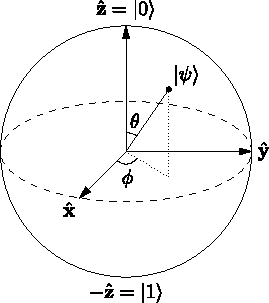
\includegraphics[width=1\textwidth]{../resources/pdfs/Bloch_Sphere.pdf}
		\end{block}
	\end{column}
\end{columns}
\end{frame}

\begin{comment}
\begin{frame}{The current state of quantum computing}
\begin{columns}[T]
	\begin{column}{.7\textwidth}
		\begin{block}{}
\begin{itemize}
	\item Though progress is slow, researchers have achieved gate based quantum computers with small numbers of qubits
	\begin{itemize}
		\item Shor's algorithm on 7 qubits
	\end{itemize}
	\item Quantum annealing, though less powerful than a universal quantum computer, shows promise
	\begin{itemize}
		\item D-Wave 2000Q has 2048 qubits
	\end{itemize}
\end{itemize}
    	\end{block}
	\end{column}
	\begin{column}{.3\textwidth}
    	\begin{block}{}
    		\includegraphics[width=1\textwidth]{dwave_2000q.jpg}
		\end{block}
	\end{column}
\end{columns}
\end{frame}

\begin{frame}{The future}
\begin{itemize}
	\item When (if?) a scalable design for gate based quantum computing is achieved, we can run Grover's algorithm
	\begin{itemize}
		\item Large speedup for many problems including NP-complete such as the traveling salesperson problem, 3-SAT
		\item Possible applications to database search
	\end{itemize}
	\item Simulation of quantum systems, chemical reactions, protein folding
	\item Quantum annealing
	\begin{itemize}
		\item Binary optimization problems
		\item Machine learning
		\item Quantum simulation
	\end{itemize}
\end{itemize}
\end{frame}
\end{comment}

\end{document}
